\section*{Resultados}
    Los parámetros de operación de las torres de destilación a partir de su simulación 
    en columnas DSTWU se muestran en las Tablas \ref{Parametros_DSTWU-1} y 
    \ref{Parametros_DSTWU-2}.

\begin{table}[H]
    \centering
    \caption{\textit{Parámetros de DSTWU-1}}
    \label{Parametros_DSTWU-1}
    \begin{tabular}{lll}
    \hline
    \multicolumn{2}{l}{DSTWU-1}                                           & Unidades \\
    \hline
    Relación mínima de reflujo                              & 1.9446      &          \\
    Relación de reflujo real                                & 2.7800      &          \\
    Número mínimo de etapas                                 & 18.2820     &          \\
    Número de etapas reales                                 & 31.8299     &          \\
    Etapa de alimentación                                   & 16.5290     &          \\
    Número de etapas reales por encima de la alimentación   & 15.5290     &          \\
    Requerimiento del hervidor                              & 129264.7000 & cal/s    \\
    Requerimiento del condensador                           & 112396.9630 & cal/s    \\
    Temperatura del destilado                               & 47.2418     & C        \\
    Temperatura inferior                                    & 81.3112     & C        \\
    Fracción para alimentación de destilado                 & 0.4468      &          \\ \hline
    \end{tabular}
\end{table}
\begin{table}[H]
    \centering
    \caption{\textit{Parámetros de DSTWU-2}}
    \label{Parametros_DSTWU-2}
    \begin{tabular}{lll}
    \hline
    \multicolumn{2}{l}{DSTWU-2}                      & Unidades    \\ \hline
    Relación mínima de reflujo         & 0.1209     &          \\
    Relación de reflujo real           & 0.8450     &          \\
    Número mínimo de etapas            & 1.7836     &          \\
    Número de etapas reales            & 2.9400     &          \\
    Etapa de alimentación              & 2.2000     &          \\
    Número de etapas reales por encima de la alimentación & 1.9448     &
    \\Requerimiento del hervidor    & 14712.0420 & cal/s \\
    Requerimiento del condensador         & 13522.2045 & cal/s  \\
    Temperatura del destilado          & 76.9745    & C        \\
    Temperatura inferior                & 94.9141    & C        \\
    Fracción para alimentación de destilado       & 0.1478     &   \\ \hline
    \end{tabular}
\end{table}

    Una vez realizada la simulación, se obtuvieron los valores que se muestran en las Tablas
    \ref{Tabla resultados}, \ref{cont_tab_3} y \ref{Continuacion resultados 2} para cada una
    de las corrientes y el gráfico que se muestra en la \textit{Figura \ref{fig:frac_mol}}. 
    Este gráfico nos muestra el número de etapas en la columna DSTL-1 y la fracción mol de acetona,
    agua, IPA e hidrógeno. La línea en color rosa nos representa la relación de fracción mol líquida 
    de acetona respecto al número de etapa, es por ello que en la etapa número uno se tiene una 
    fracción mol de aproximadamente 0.99 de acetona, ya que es por la parte superior de nuestra 
    columna por donde sale nuestra corriente de interés que es la acetona. Conforme avanza el
    número de etapas esta línea va hacia bajo hasta llegar a cero, esto se debe a que no hay
    pérdida de acetona en el fondo de nuestra columna. Por el contrario, la corriente que sale
    por el fondo y conecta a nuestra columna de destilación DSTL-2 es 0.946 fracción mol de 
    agua y 0.054 fracción mol de IPA. La segunda columna de destilación nos permite recuperar el
    IPA por la parte de arriba de nuestra columna la cual es recirculada al inicio de nuestro 
    proceso, mientras que en el fondo se obtiene una fracción mol de 0.996 de agua.

\begin{table}[H]
    \centering
    \caption{\textit{Tabla de resultados de las corrientes del proceso.}}
    \label{Tabla resultados}
    \begin{tabular}{lllllll}
    \hline
    \multicolumn{7}{l}{Reporte de corrientes}                                               \\
    \hline
    Descripción    & Unidades   & 1          & 2         & 4         & 10          & 14        \\
    \hline
    Proviene           &         & HX1        & HX2       & FLASH     & DSTL-1      & DSTL-1    \\
    Hacia             &         & HX2        & FLASH     & MIX-2     & DSTL-2      &           \\
    Fase          &         &            &           & Liquido    & Liquido      & Liquido    \\
    Temperatura    & K       & 318        & 293       & 293       & 356.2272693 & 320.39    \\
    Presión       & atm     & 1          & 1         & 1.5       & 1           & 1         \\
    Densidad    & gm/cc   & 0.0014     & 0.0025    & 0.8206    & 0.8955      & 0.7622    \\
    \textbf{Flujo molar}     & kmol/hr & 45.8038    & 45.8038   & 25.8715   & 19.7348     & 16.1244   \\
    WATER          & kmol/hr & 10.1073    & 10.1073   & 9.9230    & 18.6759     & 0.1593    \\
    IPA            & kmol/hr & 1.1010     & 1.1010    & 1.0597    & 1.0589      & 0.0376    \\
    ACETONE        & kmol/hr & 17.2977    & 17.2977   & 14.8835   & 0           & 15.9268   \\
    HYDROGEN       & kmol/hr & 17.2977    & 17.2977   & 0.0054    & 0           & 0.0007    \\
    \textbf{Frac mol} &         &            &           &           &             &           \\
    WATER          &         & 0.2207     & 0.2207    & 0.3836    & 0.9463      & 0.0099    \\
    IPA            &         & 0.0240     & 0.0240    & 0.0410    & 0.0537      & 0.0023    \\
    ACETONE        &         & 0.3776     & 0.3776    & 0.5753    & 0           & 0.9877    \\
    HYDROGEN       &         & 0.3776     & 0.3776    & 0.0002    & 0           & 0         \\
    \textbf{$\dot{m}$ másico}     & kg/hr   & 1287.7751  & 1287.7751 & 1106.8919 & 400.0852    & 930.1604  \\
    WATER          & kg/hr   & 182.0861   & 182.0861  & 178.7664  & 336.4521    & 2.8700    \\
    IPA            & kg/hr   & 66.1665    & 66.1665   & 63.6829   & 63.6330     & 2.2572    \\
    ACETONE        & kg/hr   & 1004.6523  & 1004.6523 & 864.4317  & 0.0001      & 925.0318  \\
    HYDROGEN       & kg/hr   & 34.8701    & 34.8701   & 0.0108    & 0           & 0.0013    \\
    \textbf{Frac masa} &         &            &           &           &             &           \\
    WATER          &         & 0.1414     & 0.1414    & 0.1615    & 0.8410      & 0.0031    \\
    IPA            &         & 0.0514     & 0.0514    & 0.0575    & 0.1590      & 0.0024    \\
    ACETONE        &         & 0.7801     & 0.7801    & 0.7810    & 0           & 0.9945    \\
    HYDROGEN       &         & 0.0271     & 0.0271    & 0         & 0           & 0         \\
    $\dot{Q}$   & l/min   & 15246.244 & 8637.2997 & 22.4819   & 7.4461      & 20.3397 \\  \hline
    \end{tabular}
\end{table}

\begin{table}[H]
    \centering
    \caption{\textit{Continuación Tabla 3}}\begin{tabular}{lllllll}
    \label{cont_tab_3}
    \hline
    Descripción    & 15     & AGUA     & ALIM      & GAS       & S1        & S2         \\ \hline
    Proviene            & DSTL-1 &          &           & FLASH     & ABSOR     & MIX-1      \\
     Hacia             &        & ABSOR    & MIX-1     & ABSOR     &           & VAP        \\
    Fase          & Vapor  & Liquido   & Liquido   & Vapor     & Vapor     & Liquid     \\
    Temperatura   & 320.39 & 320      & 320       & 293       & 318.7346  & 322.5447   \\
    Presión        & 1      & 1.5      & 1         & 1.5       & 1.5       & 0.9869     \\
    Densidad   & 0.0016 & 0.9726   & 0.7879    & 0.0006    & 0.0004    & 0.7874     \\
    \textbf{Flujo molar}     & 0.0223 & 10       & 25.9800   & 19.9322   & 19.9242   & 28.5061    \\
    WATER          & 0.0001 & 10       & 8.5734    & 0.1843    & 1.2731    & 10.1073    \\
    IPA            & 0      & 0        & 17.4066   & 0.0413    & 0.0047    & 18.3987    \\
    ACETONE        & 0.0161 & 0        & 0         & 2.4143    & 1.3555    & 1.36E-06   \\
    HYDROGEN       & 0.0060 & 0        & 0         & 17.2924   & 17.2910   & 0          \\
    \textbf{Frac mol} &        &          &           &           &           &            \\
    WATER          & 0.0055 & 1        & 0.3300    & 0.0092    & 0.0639    & 0.3546     \\
    IPA            & 0.0009 & 0        & 0.6700    & 0.0021    & 0.0002    & 0.6454     \\
    ACETONE        & 0.7219 & 0        & 0         & 0.1211    & 0.0680    & 4.79E-08   \\
    HYDROGEN       & 0.2717 & 0        & 0         & 0.8676    & 0.8678    & 0          \\
    $\dot{m}$ \textbf{ másico}     & 0.9492 & 180.1528 & 1200.5178 & 180.8833  & 136.7977  & 1287.7751  \\
    WATER          & 0.0022 & 180.1528 & 154.4522  & 3.3197    & 22.9345   & 182.0861   \\
    IPA            & 0.0012 & 0        & 1046.0656 & 2.4836    & 0.2805    & 1105.6889  \\
    ACETONE        & 0.9335 & 0        & 0         & 140.2206  & 78.7261   & 7.93E-05   \\
    HYDROGEN       & 0.0122 & 0        & 0         & 34.8593   & 34.8566   & 0          \\
    \textbf{Frac masa} &        &          &           &           &           &            \\
    WATER          & 0.0023 & 1        & 0.1287    & 0.0184    & 0.1677    & 0.1414     \\
    IPA            & 0.0013 & 0        & 0.8713    & 0.0137    & 0.0021    & 0.8586     \\
    ACETONE        & 0.9835 & 0        & 0         & 0.7752    & 0.5755    & 6.16E-08   \\
    HYDROGEN       & 0.0128 & 0        & 0         & 0.1927    & 0.2548    & 0          \\
    $\dot{Q}$   & 9.7558 & 3.0871   & 25.3945   & 5324.6572 & 5789.9982 & 27.2580   \\ \hline
    \end{tabular}
\end{table}

\begin{table}[H]
    \centering
    \caption{\textit{Continuación Tabla 3}}
    \label{Continuacion resultados 2}
    \begin{tabular}{llllll}
    \hline
    Descripción    & S4       & S5        & S7       & S8       & S10        \\ \hline
    Proviene             & ABSOR    & MIX-2     & DSTL-2   & DSTL-2   & VAP        \\
    Hacia              & MIX-2    & DSTL-1    &          & MIX-1    & REACT      \\
    Fase          & Liquido   &           & Liquido   & Liquido   & Vapor      \\
    Temperatura    & 303.7686 & 299.3965  & 369.6689 & 352.9200 & 389        \\
    Presión       & 1.5      & 1.5       & 0.9869   & 0.9869   & 2.6        \\
    Densidad    & 0.9178   & 0.8275    & 0.9185   & 0.7835   & 0.0037     \\
    \textbf{Flujo molar}     & 10.0080  & 35.8814   & 17.2087  & 2.5261   & 28.5061    \\
    WATER          & 8.9112   & 18.8354   & 17.1420  & 1.5339   & 10.1073    \\
    IPA            & 0.0367   & 1.0964    & 0.0667   & 0.9921   & 18.3987    \\
    ACETONE        & 1.0588   & 15.9429   & 1.16E-07 & 1.36E-06 & 1.36E-06   \\
    HYDROGEN       & 0.0014   & 0.0067    & 0        & 0        & 0          \\
    \textbf{Frac mol} &          &           &          &          &            \\
    WATER          & 0.8904   & 0.5249    & 0.9961   & 0.6072   & 0.3546     \\
    IPA            & 0.0037   & 0.0306    & 0.0039   & 0.3928   & 0.6454     \\
    ACETONE        & 0.1058   & 0.4443    & 6.76E-09 & 5.40E-07 & 4.79E-08   \\
    HYDROGEN       & 0.0001   & 0.0002    & 0        & 0        & 0          \\
    $\dot{m}$ \textbf{ másico}     & 224.2384 & 1331.1947 & 312.8279 & 87.2573  & 1287.7751  \\
    WATER          & 160.5380 & 339.3243  & 308.8182 & 27.6339  & 182.0861   \\
    IPA            & 2.2031   & 65.8914   & 4.0097   & 59.6232  & 1105.6889  \\
    ACETONE        & 61.4945  & 925.9654  & 6.75E-06 & 7.93E-05 & 7.93E-05   \\
    HYDROGEN       & 0.0027   & 0.0135    & 0        & 0        & 0          \\
    \textbf{Frac masa} &          &           &          &          &            \\
    WATER          & 0.7159   & 0.2549    & 0.9872   & 0.3167   & 0.1414     \\
    IPA            & 0.0098   & 0.0495    & 0.0128   & 0.6833   & 0.8586     \\
    ACETONE        & 0.2742   & 0.6956    & 2.16E-08 & 9.08E-07 & 6.16E-08   \\
    HYDROGEN       & 1.22E-05 & 1.02E-05  & 0        & 0        & 0          \\
    $\dot{Q}$     & 4.0721   & 26.8117   & 5.6762   & 1.8561   & 5832.7416 \\ \hline
    \end{tabular}
\end{table}
    

        \begin{figure}[H]
            \centering
            \includegraphics[scale=0.8]{images/etapas_vs_fracmol.PNG}
            \caption{Etapas vs Fracción mol de la acetona, agua, IPA e hidrógeno.}
            \label{fig:frac_mol}
        \end{figure}
    Para proponer nuestro sistema de control en el reactor mediante la relación de la 
    temperatura del reactor y la temperatura de la entrada de la chaqueta, se determinó 
    que la entrada manipulable  es la temperatura de la chaqueta $T_j$. En este caso como lo 
    indica el $\Delta H_{rxn} $ positivo, la reacción es endotérmica, por lo tanto es necesario
    calentar el reactor para llevarlo a la temperatura deseada. Con el balance de energía del 
    reactor se logró determinar la función de transferencia de nuestro proceso y mediante el 
    método de Cohen-Coon; ya que teníamos una función de transferencia a lazo abierto, se logró
    observar la estabilidad de nuestro reactor haciendo uso del software MATLAB como se muestra en 
    la Figura \ref{fig:unitario}.

\begin{table}[H]
    \caption{Valores para distintos tipos de controladores}
    \label{valore_controladores}
   \centering
   \begin{tabular}{llll}
   \hline
   Controlador & $K_c$ & $\tau_D$ & $\tau_I$  \\
   \hline
   P                   & 0.0064    & -   &-     \\
   PI                  &  0.0016  & 1.5023    & -    \\
   PID                 & 0.0048 & 7.5045   &0.0032   \\
   \hline
   \end{tabular}
\end{table}
   

        \begin{figure}[H]
            \centering
            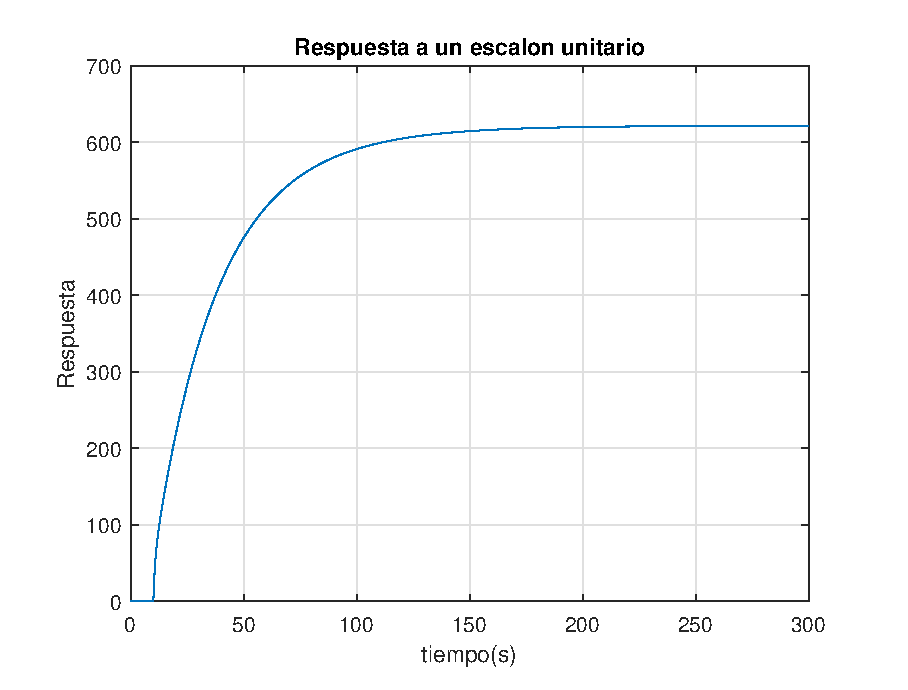
\includegraphics{images/unitarioM.eps}
            \caption{Respuesta del sistema ante un escalón unitario}
            \label{fig:unitario}
        \end{figure}

    \paragraph{}
    Para determinar la viabilidad económica del proyecto se tomó en cuenta el costo de los 
    equipos, su instalación, servicios, mano de obra operativa y de mantenimiento que nos 
    ofrece el análisis económico de Aspen que se muestra en las Tablas \ref{tab:equipos}, 
    \ref{tab:servicios}, \ref{tab:serviciosxaño}, \ref{tab:manodeobra} y \ref{tab:resultados}, 
    por nuestra parte determinamos el costo total de la materia prima y con base en el 
    análisis de mercado se determinaron las ventas totales del producto, una vez determinada 
    la tasa de retorno TIR se obtiene una tasa positiva lo cual indica que hemos tenido unos 
    beneficios mayores a la inversión realizada y por tanto hemos obtenido ganancias.
    \paragraph{}

\begin{table}[H]
    \centering
    \caption{Costo de equipos e instalación}
    \label{tab:equipos}
    \begin{tabular}{l|r|r}
    \hline
    \multicolumn{1}{c|}{Equipo} & \multicolumn{1}{c|}{Costo (USD)} & \multicolumn{1}{c}{Costo de instalación (USD)} \\ \hline
    Vaporizador                 & 15,600.00                        & 103,100.00                                     \\
    Reactor                     & 100,000.00                       & 250,000.00                                     \\
    Enfriador                   & 9,900.00                         & 99,600.00                                      \\
    Condensador                 & 10,000.00                           & 66,500.00                                      \\
    Separador flash             & 15,600.00                           & 96,000.00                                      \\
    Columna de absorción        & 41,300.00                           & 169,500                                        \\
    Columna de destilación 1    & 233,200.00                       & 652,600.00                                     \\
    Columna de destilación 2    & 56,900.00                           & 382,400.00                                     \\ \hline
    Total                       & 482,500.00                       & 1,819,700.00     \\ \hline                             
    \end{tabular}
\end{table}

\begin{table}[H]
    \centering
    \caption{Servicios}
    \label{tab:servicios}
    \hline 
    \resizebox{\textwidth}{!}{%
    \begin{tabular}{l|l|cc|c}
    \multicolumn{1}{c|}{Nombre} & \multicolumn{1}{c|}{Fluido} & Velocidad & Unidades de velocidad & Costo por hora (USD/H) \\ \hline
    Electricidad                &                             & 53.532    & KW                    & 4.14873                \\
    Agua de enfriamiento        & Agua                        & 0.019092  & MMGAL/H               & 2.29104                \\
    Refrigerante - Freon 12     & Refrigerante                & 8.414624  & KLB/H                 & 0.715243               \\
    Vapor 100PSI               & Vapor                       & 2.532263  & KLB/H                 & 20.612621 \\ \hline             
    \end{tabular}%
    }
\end{table}

\begin{table}[H]
    \centering
    \caption{Costo de servicios por año}
    \label{tab:serviciosxaño}
    
    \begin{tabular}{l|c}
    \hline 
      Servicio                    & \multicolumn{1}{l}{USD/año} \\ \hline
    Electricidad          & 36,367.8                      \\
    Servicios del proceso & 207,043                       \\ \hline
    Total                 & 243,411  \\ \hline                     
    \end{tabular}
\end{table}
    

    

\begin{table}[H]
    \centering
    \caption{Costo de mano de obra operativa y mantenimiento}
    \label{tab:manodeobra}
    \begin{tabular}{l|l|l}
    \hline 
    \textbf{Mano de obra}  &                    &            \\ \hline 
    Operadores por turno   &                    & 2          \\
    Costo unitario         & Costo/Operador/h   & 20         \\ \hline
    Total (USD)            & Costo/año          & 350,640.00 \\
                           &                    &            \\ \hline 
    \textbf{Mantenimiento} &                    &            \\ \hline 
    Costo/8000 h           &                    & 29100      \\ \hline 
    Total (USD)            & Costo/año          & 31,886.3   \\
                           &                    &            \\ \hline 
    \textbf{Supervisión}   &                    &            \\ \hline 
    Supervisores por turno &                    & 1          \\
    Costo unitario         & Costo/Supervisor/h & 35         \\ \hline
    Total (USD)                 & Costo/año          & 306,810   \\ \hline 
    \end{tabular}
\end{table}

\begin{table}[H]
    \centering
    \caption{Resumen de resultados del proyecto}
    \label{tab:resultados}
    \begin{tabular}{l|c} \hline 
    Costo de capital total del proyecto  [USD]                               & 5,673,990  \\
    Costo total de operación   [USD/año]                        & 1,557,120   \\
    Costo total de mano de obra operativa y mantenimiento [USD] & 689,336     \\
    Costo total de materia prima   [USD/año]                    & 708,644          \\
    Ventas totales de producto [USD/año]                        & 13,320,400
    
              \\
    Costo total de servicios   [USD/año]                        & 243,411     \\
    Costo de equipo [USD]                                       & 482,500     \\
    Costo total de instalación [USD]                            & 1,819,700 \\ \hline   
    \end{tabular}
\end{table}

    La tasa  de retorno TIR  a un periodo de 2 años es de:
    \textbf{2.104}

        $$0 = - 5,673,990 + \dfrac{13,320,400}{1+TIR} +\dfrac{13,320,400}{(1+TIR)^2}  $$
    Despejando para TIR se obtiene los 2.104 